The following two chapters consider the impact of using emering NVRAM technologies for durable transaction processing.
Refer to Section~\ref{sec:Background:Storage:NVRAM} for an overview of storage technologies and Section~\ref{sec:Background:Recovery} for a description of ARIES, a popular recovery mechanism for disk.
Work relating to the next two chapters is currently under review at VLDB.
I completed this work under the advisement of my advisor, Thomas F. Wenisch, and collaborators at Oracle, Brian T. Gold and Bill Bridge.
I was the sole graduate student and technical contributer (programming and running experiments) for the project, although my co-authors were vital to development the following ideas.
I would especially like the thank Brian and Bill for bringing industry's point of view and ``real world" examples to this collaboration.

This chapter outlines the problems with existing disk recovery management, the potential pitfalls of using NVRAM for persistent applications, a methodology for evaluating NVRAM devices that do not yet exist, and a description of several candidate software designs for NVRAM recovery management, to be evaluated later.
I consider this chapter largely complete with two exceptions.
First, I have performed a validation of my timing model that has not yet been published that I intend to include in the final thesis \fixme{forward ref a section}.
Second, my implementation of \GroupCommit is more complex (and interesting, in my opinion) than a 12 page journal paper allows room to describe.
I intend to include a detailed description in Section \fixme{forward ref}.

\section{Introduction}
\label{sec:OLTP_design:Intro}

Emerging nonvolatile memory technologies (NVRAM) offer an alternative to disk that is persistent, provides read latency similar to DRAM, and is byte-addressable \cite{BurrKurdi08}.
Such NVRAMs could revolutionize online transaction processing (OLTP), which today must employ sophisticated optimizations with substantial software overheads to overcome the long latency and poor random access performance of disk.
Nevertheless, many candidate NVRAM technologies exhibit their own limitations, such as greater-than-DRAM latency, particularly for writes \cite{LeeIpek09}.

These NVRAM technologies stand to revolutionize Online Transaction Processing (OLTP), where consistency and durability are paramount, but applications demand high throughput and low latency.
Prior work has already demonstrated the potential of these technologies to enhance file systems \cite{GreenanMiller06, ConditNightingale09} and persistent data structures \cite{VenkataramanTolia11}, but has not considered OLTP. 
Today, OLTP systems are designed from the ground up to circumvent disk's performance limitations.
For example, many popular database systems use Write-Ahead Logging (WAL; e.g., ARIES \cite{MohanHaderle92}) to avoid expensive random disk writes by instead writing to a sequential log.  
Although effective at hiding write latency, WAL entails substantial software overheads.

NVRAM offers an opportunity to simultaneously improve database forward-processing throughput and recovery latency by rethinking mechanisms that were designed to address the limitations of disk.
Figure~\ref{fig::Recovery} demonstrates this potential, displaying recovery time and transaction throughput for the TPCB workload running on the Shore-MT storage manager \cite{JohnsonPandis09} for hypothetical NVRAM devices (see Section~\ref{sec:OLTP_design:Methodology} for a description of the methodology).

\begin{figure}
  \centering
  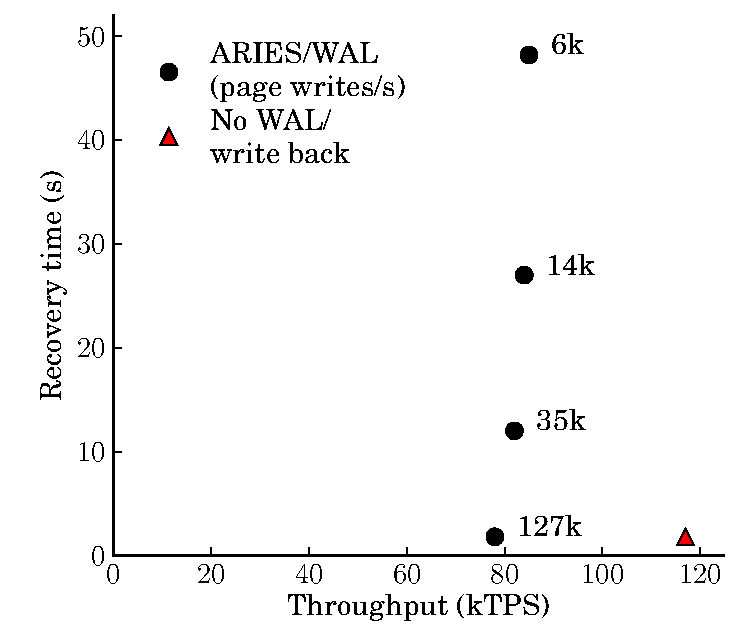
\includegraphics[width=.6\linewidth]{OLTP_design/TPCB_Recovery.pdf}
  \caption{\textbf{TPCB recovery latency vs throughput.} Increasing page flush rate reduces recovery latency.  Removing WAL entirely improves throughput by 50\%.}
  \label{fig::Recovery}
\end{figure}


The ARIES/WAL points (black circles) in the Figure show forward-processing throughput (horizontal axis) and recovery time (vertical axis) as a function of device write throughput (annotated alongside each point).
As database throughput can greatly outpace existing storage devices (this configuration requires 6,000 page writes/s to bound recovery at maximum transaction throughput; measured disk and flash devices provide only 190 and 2,500 page writes/s, respectively) I model recovery performance under faster NVRAM using a RAM disk for log and store while limiting the page flush rate.
As intuition would suggest, greater write bandwidth enables more aggressive flushing, minimizing the number of dirtied pages in the buffer cache at the time of failure, reducing recovery time.
With enough write bandwidth (in this case, 127,000 flushes/s, or 0.97 GB/s random writes for 8KB pages) the database recovers near-instantly, but forward-processing performance remains compute bound.
Achieving such throughput today requires large, expensive disk arrays or enterprise flash storage devices; future NVRAM devices might enable similar performance on commodity systems.

NVRAM opens up even more exciting opportunities for recovery management if we consider re-architecting database software.
The Figure shows this additional potential with a design point (red triangle) that removes WAL and asynchronous page flushing---optimizations primarily designed to hide disk latency.
Throughput improves due to three effects: (1) threads previously occupied by page and log flushers become available to serve additional transactions, (2) asynchronous page flushing, which interferes with transactions as both flusher and transaction threads latch frequently accessed pages, is removed, and (3) transactions no longer insert WAL log entries, reducing the transaction code path.
In aggregate these simplifications amount to a 50\% throughput increase over ARIES's best possible NVRAM performance.
The key take-away is that database optimizations long used for disk only hinder performance with faster devices.
In this chapter, I investigate how to redesign durable storage and recovery management for OLTP to take advantage of the low latency and byte-addressability of NVRAM.

NVRAMs, however, are not without their limitations.
Se\-veral candidate NVRAM technologies exhibit larger read latency and significantly larger write latency compared to DRAM.
Additionally, whereas DRAM writes benefit from caching and typically are not on applications' critical paths, NVRAM writes must become persistent in a constrained order to ensure correct recovery.
I consider an NVRAM access model where correct ordering of persistent writes is enforced via \emph{persist barriers}, which stall until preceding NVRAM writes are complete; such persist barriers can introduce substantial delays when NVRAM writes are slow.

This chapter outlines an approach to architecting recovery management for transaction processing using NVRAM technologies
I discuss potential performance problems with using NVRAM and possible software architectures to address these problems.
Additionally, I propose an evaluation framework, involving memory trace analysis, code annotation, and precise timing models for OLTP running on existing hardware platforms.
Subsequent chapters will build on the designs and methodology presented here to determine when OLTP must be redesigned and what problems might remain.

\section{Recovery Management Design}
\label{sec:OLTP_design:Design}

\begin{table*}
  \footnotesize
  \centering
  \renewcommand{\arraystretch}{2.5}
  \begin{tabular*}{\textwidth}{l l l l}
     & \pbox{1.1 in}{\emph{NVRAM\newline Disk-Replacement}} & \pbox{1.5 in}{\InPlace} & \pbox{1.5 in}{\GroupCommit} \\
    \emph{Software buffer} & \cellcolor[gray]{.8}\pbox{1.1 in}{Traditional WAL/ARIES} & \cellcolor[gray]{.8}\pbox{1.5 in}{Updates both buffer and NVRAM} & \cellcolor[gray]{.8}\pbox{1.5 in}{Buffer limits batch size} \\
    \emph{Hardware buffer} & \cellcolor[gray]{.95}\pbox{1.1 in}{Impractical} & \cellcolor[gray]{.95}\pbox{1.5 in}{Slow uncached NV\-RAM reads} & \cellcolor[gray]{.95}\pbox{1.5 in}{Requires hardware support} \\
    \emph{Replicate to DRAM} & \multicolumn{3}{l}{\pbox{4.1 in}{\cellcolor[gray]{.8}Provides fast reads and removes buffer management, but requires large DRAM capacity}} \\
  \end{tabular*}
  \caption{\textbf{NVRAM design space.} Database designs include recovery mechanisms (top) and cache configurations (left).}
  \label{table::DesignSpace}
\end{table*}


Near-future NVRAM devices will undoubtedly be faster than both disk and flash.
However, compared to DRAM many NVRAM technologies impose slower reads and significantly slower persistent writes.
We must consider both in redesigning OLTP for NVRAM.

\subsection{NVRAM Reads}
\label{sect:OLTP_design:Design:Reads}
While the exact read performance of future NVRAM technologies is uncertain, many technologies and devices increase read latency relative to DRAM.
Current databases and computer systems are not equipped to deal with this read latency.
Disk-backed databases incur sufficiently large read penalties (on the order of milli-seconds) to justify software-managed DRAM caches and buffer management.
On the other hand, main-memory databases rely only on the DRAM memory system, including on-chip data caches.
Increased memory latency and wide-spread data accesses may require hardware or software-controlled DRAM caches even when using byte addressable NVRAM.

I consider three configurations of cache management; these alternatives form the three rows of Table~\ref{table::DesignSpace} (subsequent sections consider the recovery management strategies, forming the three columns).
The first option, \emph{Software Buffer}, relies solely on software to manage a DRAM buffer cache, as in conventional disk-backed database systems.
The cache may be removed entirely or execution relies soly on a \emph{Hardware Buffer}, as in main-memory databases.
Hardware caches are fast (e.g., on-chip SRAM) and remove complexity from the software, but provide only limited capacity.
Third, one might \emph{replicate to DRAM} all data that is stored in NVRAM---all writes update both DRAM and NVRAM (for recovery), but reads retrieve data exclusively from DRAM.
Replicating data ensures fast reads by avoiding increased NVRAM read latencies (except for recovery) and simplifies buffer management, but requires large DRAM capacity.

\subsection{NVRAM Writes}
\label{sec:OLTP_design:Design:Writes}

Persistent writes, unlike reads, do not benefit from cach\-ing; writes persist through to the device for recovery correctness.
Additionally, NVRAM updates must be carefully ordered to ensure consistent recovery.
I assume that ordering is enforced through a generic mechanism called a \emph{persist barrier}, which guarantees that writes before the barrier persist before any dependant operations after the barrier persist.

Persist barriers may be implemented in several ways.
The easiest, but worst performing, is to delay threads that issue persist barriers until all pending NVRAM writes successfully persist.
More complicated mechanisms improve performance by allowing threads to continue executing beyond the persist barrier and only delaying thread execution when persist conflicts arise (i.e., a thread reads or overwrites shared data from another thread that has not yet persisted).
BPFS provides an example implementation of this mechanism \cite{ConditNightingale09}.
Regardless of how they are implemented, persist barriers can introduce expensive synchronous delays on transaction threads; the optimal recovery mechanism depends on how expensive, on average, persist barriers become.
To better understand how persist barriers are used and how frequently they occur, I outline operations to atomically update persistent data using persist barriers, and use these operations to implement three recovery mechanisms for NVRAM.

\textbf{Atomic durable updates.}
{
\singlespacing
\newsavebox{\persistwal}
\begin{lrbox}{\persistwal}
\begin{lstlisting}
persist_wal(log_buffer, nvram_log)
  for entry in log_buffer:
    nvram_log.force_last_lsn_invalid(entry)
    nvram_log.insert_body(entry) # no lsn
  persist_barrier()
  nvram_log.update_lsns()
  persist_barrier()
\end{lstlisting}
\end{lrbox}

\newsavebox{\persistpage}
\begin{lrbox}{\persistpage}
\begin{lstlisting}
persist_page(page_v, page_nv, page_log)
  page_log.copy_from(page_nv)
  persist_barrier()
  page_log.mark_valid()
  persist_barrier()
  page_nv.copy_from(page_v)
  persist_barrier()
  page_log.mark_invalid()
  persist_barrier()
\end{lstlisting}
\end{lrbox}

\begin{figure}[]
  \subfigure{ \usebox{\persistwal} }
  \subfigure{ \usebox{\persistpage} }

  \caption{\textbf{Durable atomic updates.} \texttt{persist\_wal()} appends to the ARIES log using two persist barriers.  \texttt{persist\_page()} persists pages with four persist barriers.}
  \label{fig::Code}
\end{figure}
}

Figure~\ref{fig::Code} shows two operations to atomically update NVRAM data.
The first, \texttt{persist\_wal()}, persists log entries into an ARIES log.
Sho\-re-MT log entries are post-pended with their Log Serial Number (LSN -- log entry file offset).
At recovery, a log entry is considered valid only if this tail LSN matches the location of the entry.
I persist log entries atomically by first persisting an entry without its tail LSN, and only later (once we are certain the entry is persistent) persist the LSN.
This order is enforced by inserting a persist barrier between writing the log entry and its LSN.
Additionally, I reduce the number of persist barriers by persisting entries in batches, writing several log entries at once (without LSNs), followed by all their LSNs, separated by a single persist barrier.
It is entirely possible (yet unlikely) that pre-existing LSN tails already match the log entry's offset; tails must be checked and first reset when this occurs.
Log operations introduce two persist barriers---one to ensure that log entries persist before their LSNs, and one to enforce that LSNs persist before the thread continues executing.

The second operation, \texttt{persist\_page()}, atomically persists page data with the use of a persistent undo page log.
First, the page's original data is copied from NVRAM to the page log.
The page log is marked valid and the dirty version of the page is copied to NVRAM (or updated in-place while locks are held).
Finally, the log is marked invalid.
Four persist barriers ensure that each update persists before the next, enforcing consistency at all points in execution.
Recovery checks the valid flags of all page logs, copying any valid log back in-place.
The log is always valid while the page persists in-place, protecting against partial NVRAM writes.
Together, \texttt{persist\_wal()} and \texttt{persist\_page()} provide the tools necessary to construct recovery mechanisms.
I discuss these mechanisms next, describing their implementation and performance.

\textbf{NVRAM Disk-Replacement.}
NVRAM database systems will likely continue to rely on ARIES/WAL at first, using NVRAM as \NVDisk.
WAL provides recovery for disk by keeping an ordered log of all updates, as described in Section~\ref{sec:Background:Recovery}.
While retaining disk's software interface, NVRAM disk accesses are implemented as copies between the volatile and nonvolatile address spaces.
\NVDisk in Shore-MT persists the log and pages with \texttt{persist\_wal()} and \texttt{persist\_page()}, respectively.
However, persists occur on log and page flusher threads, and transaction threads do not observe persist barrier delays (except when waiting for commit log entries to persist).
\NVDisk provides low recovery latency by aggressively flushing pages, minimizing the size of data to recover.
While requiring the least engineering effort, \NVDisk contains large software overheads to maintain a centralized log and asynchronously flush pages.
Next, I leverage NVRAM's low latency to reduce these overheads.

\textbf{In-Place Updates.}
Fast, byte-addressable NVRAM allows updates to persist in-place and enforce persist order immediately, a design we call \InPlace.
\InPlace allows us to remove the centralized log by replacing redo and undo log functionality elsewhere.
I remove redo logs by keeping the database's durable state up-to-date.
In ARIES terms, the database is constantly at its replayed state---there is no need to replay a redo log after failure.
Undo logs need not maintain a global order (transactions are already free to roll back in any order), and instead I distribute ARIES undo logs per transaction.
Such non-concurrent logs are simpler and impose less overhead than centralized logs.
Other databases (such as Oracle) already distribute undo logs in rollback segments \fixme{cite}.
Transaction undo logs remain durable so that in-flight transactions at the time of failure can be rolled back.
Each page update consists of (1) latching the page, (2) inserting an undo entry into the transaction-private undo log, using \texttt{persist\_wal()}, (3) updating the page in-place, using \texttt{persist\_page()} (without an intermediate volatile page), and (4) releasing the page latch.
This protocol ensures all updates to a page, and updates within a transaction, persist in-order, and that no transaction reads data from a page until it is durable.
Recovery applies undo logs for in-flight transactions; there is no need to replay a redo log.

Persisting data in-place removes expensive redo logging and asynchronous page flushing, but introduces persist barriers on transactions' critical paths.
For sufficiently short persist barrier delays \InPlace outperforms \NVDisk (if persist barrier delays are negligible \InPlace resembles existing non-recoverable in-memory databases).
However, one would expect transaction performance to suffer as persist barrier delay increases.

In response, I introduce \GroupCommit, a recovery mechanisms designed to minimize the frequency of persist barriers while still removing WAL.
\GroupCommit is an entirely new design, committing instructions in large batches to minimize persist synchronization.
The next section describes, in detail, the operation and data structures necessary to implement \GroupCommit.

\section{NVRAM Group Commit}
\label{sec:OLTP_design:GroupCommit}

The two previous recovery mechanisms provide high throughput under certain circumstances, but also fail to perform in others.
\NVDisk is insensitive to large persist barrier delays as it was originally designed for disk.
However, it assumes IO delays to be the dominant performance bottleneck and trades off software overhead to minimize IO.
\InPlace, on the other hand, excels when persist barriers delays are short.
As persist barrier latency increases performance suffers, such that \NVDisk eventually performs better.
Here, I provide a third option, coupling \NVDisk's persist barrier latency-insensitivity with \InPlace's low software overhead: \GroupCommit.

\subsection{Description}
\label{sec::OLTP_design:GroupCommit:Proposed}

\GroupCommit operates by executing transactions in batches, whereby all transactions in the batch commit or (on failure) all transactions abort.
Transactions quiesce between batches, allowing only transactions from the oldest batch to execute.
Each transaction maintains a private ARIES-style undo log, supporting abort and roll-back as in \InPlace, but transaction logs are no longer persistent.
ARIES undo logs support concurrent durable transactions.
As batches persist atomically, transactions no longer roll back selectively during recovery, obviating the need for persistent ARIES undo logs.
Instead, recovery relies on a database-wide undo log and staging buffer to provide durable atomic batches.

\GroupCommit limits persist barrier frequen\-cy by enforcing persistence by batch rather than by transaction.
Persisting a batch resembles \texttt{persist\_page()}, used across the entire database, once per batch.
Because undo logging is managed at the batch level, transactions' updates may not persist in-place to NVRAM until all transactions in the batch complete.
Rather, transactions write to a volatile staging buffer, tracking dirtied cache lines in a concurrent bit field.
The bit field facilities quickly finding all dirtied data at batch completion.
Once the batch ends and all transactions complete, the pre-batch version of dirtied data is copied to the database-wide persistent undo log, only after which is data copied from the staging buffer in-place to NVRAM.
Finally, the database-wide undo log is invalidated, transactions commit, and transactions from the next batch begin executing.
%Batching allows NVRAM persists to coalesce -- the log persists only the earliest version of data from the batch, while only the last version of data persists in-place, with intermediate values never persisting.
On failure the log is copied back to the NVRAM database, aborting and rolling back all transactions from the in-flight batch.
The key observation is that \GroupCommit persists entire batches of transactions using four persist barriers, far fewer than required with \InPlace.  Note, however, that it enables recovery only to batch boundaries, rather than transaction boundaries.

I briefly outline two implementation challenges: long transactions and limited staging buffers.
Long transactions present a problem by forcing all other transactions in the batch to defer committing until the long transaction completes.
Limited staging buffers, not large enough to fit the entire data set, may fill while transactions are still executing.
I solve both problems by resorting to persistent ARIES-style undo logs, as in \InPlace.
Long transactions persist their ARIES undo log (previously volatile), allowing the remainder of the batch to persist and commit.
The long transaction joins the next batch, committing when that batch commits.
At recovery the most recent batch rolls back, and the long transaction's ARIES undo log is applied, removing updates that persisted with previous batches.
Similarly, if the staging buffer fills, the current batch ends immediately and all outstanding transactions persist their ARIES undo logs.
The batch persists, treating any in-flight transactions as long transactions, reassigning them to the next batch.
Transaction-local ARIES undo logs invalidate as the batch commits, requiring additional persistent data structures to allow transaction and batch logs to invalidate atomically.

\GroupCommit requires fewer persist barriers than \InPlace yet avoids expensive logging found in \NVDisk.
A batch requires only four persist barriers, regardless of batch length.
Expensive persist barrier delays can be amortized over additional transactions by increasing batch length, improving throughput.
Batch length must be at least large enough to amortize time spent quiescing transactions between batches.
However, increasing batch length defers commit for all transactions in the batch, increasing transaction latency.

\subsection{Proposed Work}
\label{sec::OLTP_design:GroupCommit:Proposed}

\GroupCommit only improves throughput so long as the time between batches to quiesce transactions, locate dirtied data, and persist that data is substantially less than time during each batch where transactions execute.
To provide a fair comparison between recovery mechanisms, I implement a true version of \GroupCommit in Shore-MT.
Whereas I expect NVRAM to have sufficient bandwidth to persist data quickly, orchestrating data copies, tracking dirty data with low overhead, and locating dirty data efficiently proved to be difficult software problems.
The details of this implementation were omitted from the VLDB submission, but are included here, including work to be done.

\textbf{Concurrent Dirty Set.}
As described previously, \GroupCommit requires each batch to track dirty data.
This is done with an efficient concurrent set, tracking the set of buffer pool cache lines dirtied by each batch.
In order to maximize transaction throughput, this set must allow low overhead updates by concurrent threads during batch execution, and fast iteration during batch persist.

The first attempt to create a set used an STL \emph{ordered\_set} (implemented as a balanced tree).
However, inserting cache lines to the dirty set was prohibitively expensive, slowing transactions down.
On the other hand, \emph{ordered\_set} allows relatively fast iteration over the dirty set during batch copy.
The next attempt used a bitmap of dirty cache lines, each bit corresponding to a cache line in the buffer pool.
A 10GB buffer pool requires 20MB of bits to track dirty cache lines.
Before each batch starts, after the previous batch finishes persisting, dirty bits must be flash cleared in order to track the next batch.
While bits can be quickly updated via an atomic OR operation, iterating over the dirty bits during persist was too slow, requiring a different solution.

Instead, I leveraged the fact that dirty regions were rare and sparsely located throughput the buffer pool.
Batches contain up to thousands of transactions, yet these transactions could only manage to write to a small portion of a 10GB buffer pool.
It is therefore necessary to efficiently skip over large regions of clean data when iterating through the dirty set.
To achieve this, I created a \emph{tiered bitfield set}.
The tiered bitfield set contains two bitfield sets.
The first is as described above, where each bit corresponds to a cache line in the buffer pool.
In addition, there is a higher level bit field, each bit corresponding to a \emph{cache line of the primary bit field}.
Thus, a set bit in the top level bit field indicates that some bit within a cache line of the primary bit field is set, which in turn corresponds to dirty cache line in the buffer pool.

Updating this set requires atomic OR on the necessary bits in both bit fields of the set, a small cost.
Iterating over the set now involves iterating over the (much smaller) top level bit field, finding \emph{segments} of the primary bit field known to contain at least one set bit.
This iteration reduces both the number of instructions and cache/memory lines accessed, minimizing persist time between batches.

I propose to include additional work demonstrating the sparse nature of writes to the buffer pool, as well as timing results that show that fast dirty line tracking and persist is possible.

\textbf{Concurrent Persist.}
I have shown that dirty lines can be tracked and iterated over efficiently.
However, persisting each batch with the batch coordinator alone results in long persist delays.
These delays are due to the \emph{software} overhead of copying data, not from NVRAM limitations.
To reduce these delays all persist operations must be parallelized across threads.
Luckily, we have threads to spare -- transaction threads that have quiesced between batches.
Instead of sitting idle, these threads now participate in persisting each batch.

The buffer pool address space and corresponding portions of the dirty line set are partitioned into several segments, each placed in a task queue.
The batch coordinator and transaction threads blocked by the persist process each participate by accepting tasks to persist buffer pool partitions (both log and then data in-place).
Once all tasks complete the batch commits, allowing the next batch to begin.

I propose to include results showing that persist parallelization is necessary, but is an effective way to accelerate batching.

Once both of these optimizations are implemented the system is using all cores to persist, and profiling shows that \emph{memcpy} operations, copies from the buffer pool to the persistent address space, are the primary bottleneck (memcpy is implemented using fast SSE instructions and cannot be optimized further).
Persist time is minimized, and there is little room left for improvement.

\section{Design Space}
\label{sec:OLTP_design:Designs}
I describe the space of possible designs given choices regarding NVRAM read and write performance.
This discussion ignores possible uses of hard disk to provide additional capacity.
Each design works alongside magnetic disk with additional buffer management and the constraint that pages persist to disk before eviction from NVRAM.

Table~\ref{table::DesignSpace} lists the possible combinations of caching architectures and recovery mechanisms.
The left column presents \NVDisk, which we see as the obvious and most incremental use for NVRAM.
Of note is the center-left cell, \NVDisk without the use of a volatile buffer.
WAL, by its design, allows pages to write back asynchronously from volatile storage.
Removing the volatile cache requires transactions to persist data in-place, but do so only after associated log entries persist, retaining the software overheads of \NVDisk as well as the frequent synchronization in \InPlace.
Thus, this design is impractical.

The middle-column recovery mechanism, \InPlace, represents the most intuitive use of NVRAM in database systems, as noted in several prior works.
Agrawal and Jagadish explore several algorithms for atomic durable transactions with an NVRAM main-memory \cite{AgrawalJagadish89}.
They describe the operation and correctness of each mechanism and provide an analytic cost model to compare them.
Their work represents the middle column, middle row of Table~\ref{table::DesignSpace} (\InPlace with no volatile buffer).
Aky\"{u}rek and Salem present a hybrid DRAM and NVRAM buffer cache design alongside strategies for managing cache allocation \cite{SalemAkyrek95}.
They evaluate their allocation strategies using database traces and queuing models to demonstrate the effectiveness of NVRAM at accelerating persistent writes.
Partial Memory Buffers is closest to the middle-top cell of the design space table (\InPlace with a software-managed DRAM buffer), although that design considers NVRAM as part of a hybrid buffer, not the primary persistent store.
None of these works considers alternative approaches (such as \GroupCommit), to account for large persist barrier latency and associated delays.
Additionally, This work extends prior work by providing a more precise performance evaluation and more detailed consideration of NVRAM characteristics.

The right column presents \GroupCommit.
I am not aware of any previous work that extends disk group commit to reduce the frequency of NVRAM persist barriers.
A limited-capacity staging buffer (i.e., one insufficient for the entire data set) may limit batch size, as described above.

Each of the three recovery mechanisms may replicate all data between NVRAM and DRAM to ensure fast read accesses, manage a smaller DRAM buffer cache, or omit the cache altogether.
In Section~\ref{section::Reads} I consider the importance of NVRAM caching to transaction throughput.
Then, in Section~\ref{section::Persists} I assume a DRAM-replicated data store to isolate read performance from persist performance in evaluating each recovery mechanisms's ability to maximize transaction throughput.
The next section describes an evaluation methodology for OLTP on NVRAM.

\section{Methodology}
\label{sec:OLTP_design:Methodology}

This section details the methodology for benchmarking transaction processing and modeling NVRAM performance.
Experiments use the Shore-MT storage manager \cite{JohnsonPandis09}, including the high performance, scalable WAL implementation provided by Aether \cite{JohnsonPandis10}.
While Aether provides a distributed log suitable for multi-socket servers, the distributed log exists as a fork of the main Shore-MT project.
Instead, I limit experiments to a single CPU socket to provide a fair comparison between WAL and other recovery schemes, enforced using the Linux \emph{taskset} utility.
Experiments place both the Shore-MT log and volume files on an in-memory \emph{tmpfs}, and provide sufficiently large buffer caches such that all pages hit in the cache after warmup.
The intent is to allow the database to perform data accesses at DRAM speed and introduce additional delays to model NVRAM performance.
Table~\ref{table::Specs} shows the experimental system configuration.

\begin{table}
  \centering
  \begin{tabular}{l l}
    \hline
    Operating System & Ubuntu 12.04 \\
    CPU & Intel Xeon E5645 \\
    & 2.40 GHz \\
    CPU cores & 6 (12 with HyperThreading) \\
    Memory & 32 GB \\
    \hline
  \end{tabular}
  \caption{\textbf{Experimental system configuration.}}
  \label{table::Specs}
\end{table}

\textbf{Modeling NVRAM delays.}
Since NVRAM devices are not yet available, we must provide a timing model that mimics their expected performance characteristics.
I model NVRAM read and write delays by instrumenting Shore-MT with precisely controlled assembly-code delay loops to model additional NVRAM latency and bandwidth constraints at 20ns precision.
Hence, Shore-MT runs in real time as if its buffer cache resided in NVRAM with the desired read and write characteristics.

I introduce NVRAM read and write delays separately.
Accurately modeling per-access increases in read latency is challenging, as reads are frequent and the expected latency increases on NVRAM are small.
It is infeasible to use software instrumentation to model such latency increases at the granularity of individual reads; hardware support, substantial time dilation, or alternative evaluation techniques (e.g., simulation) would be required, all of which compromise accuracy and the ability to run experiments at full scale.
Instead, I use offline analysis with PIN \cite{LukCohn05} to determine (1) the reuse statistics of buffer cache pages, and (2) the average number of cache lines accessed each time a page is latched.
Together, these offline statistics provide an average number of cache line accesses per page latch event in Shore-MT while considering the effects of page caching.
I then introduce a delay at each latch based on the measured average number of misses and an assumed per-read latency increase based on the NVRAM technology.

I model NVRAM persist delays by annotating Shore-MT to track buffer cache writes at cache line granularity---64 bytes---using efficient ``dirty" bitmaps.
Depending on the recovery mechanism, we introduce delays corresponding to persist barriers and to model NVRAM write bandwidth contention.
Tracking buffer cache writes introduces less than a 3\% overhead to the highest throughput experiments.

I create NVRAM delays using the x86 RDTSCP instruction, which returns a CPU-frequency-invariant, monotonically increasing time-stamp that increments each clock tick.
RDTSCP is a synchronous instruction---it does not allow other instructions to reorder with it.
The RDTSCP loop delays threads in increments of 20ns (latency per loop iteration and RDTSCP) with an accuracy of 2ns.

In addition to NVRAM latency, I model shared NVRAM write bandwidth.
Using RDTSCP as a clock source, I maintain a shared \emph{next\_available} variable, representing the next clock tick in which the NVRAM device is available to be written.
Each NVRAM persist advances \emph{next\_available} to account for the latency of its persist operation.
Reservations take the maximum of \emph{next\_available} and the current RDTSCP and add the reservation duration.
The new value is atomically swapped into \emph{next\_available} via a Compare-And-Swap (CAS).
If the CAS fails (due to a race with a persist operation on another thread), the process repeats until it succeeds.
Upon success, the thread delays until the end of its reservation.
The main limitation of this approach is that it cannot model reservations shorter than the delay required to perform a CAS to a contended shared variable.
This technique models reservations above 85ns accurately, which is sufficient for my experiments.

I choose on-line timing modeling via software instrumentation in lieu of architectural simulations to allow experiments to execute at full scale and in real time.
While modeling aspects of NVRAM systems such as cache performance and more precise persist barrier delays require detailed hardware simulation, I believe NVRAM device and memory system design are not sufficiently established to consider this level of detail.
Instead, I investigate more general trends to determine if and when NVRAM read and write performance warrant storage management redesign.

\textbf{Recovery performance.} Figure~\ref{fig::Recovery} displays recovery latency vs transaction throughput for the TPCB workload, varying page flush rate.
Page flush rate is controlled by maintaining a constant number of dirty pages in the buffer cache, always flushing the page with the oldest volatile update.
Experiments run TPCB for one minute (sufficient to reach steady state behavior) and then kill the Shore-MT process.
Before starting recovery I drop the file system cache.
Reported recovery time includes only the recovery portion of the Shore-MT process; I do not include system startup time nor non-recovery Shore-MT startup time.

\textbf{Workloads}
I use three workloads and transactions in this evaluation: TPCC, TPCB, and TATP.
TPCC models order management for a company providing a product or service \cite{TPCC}.
TPCB contains one transaction class and models a bank executing transactions across branches, tellers, customers, and accounts \cite{TPCB}.
TATP includes seven transactions to model a Home Location Registry used by mobile carriers \cite{TATP}.
Table~\ref{table::Workloads} shows the workload configuration.
I choose a single updating transaction from each workload and size workloads to fit in a 12GB buffer cache.
All experiments report throughput as thousands of Transactions Per Second (kTPS).
Experiments perform ``power runs" -- each thread generates and executes transactions continuously without think time -- and run an optimal number of threads per configuration (between 10 and 12).

\begin{table}
  \centering
  \begin{tabular}{l l l l}
    \hline
    Workload & Scale factor & Approx. size & Transaction \\
    \hline \hline
    TPCC & 70 & 9GB & New order \\
    TPCB & 1000 & 11GB & TPCB \\
    TATP & 600 & 10GB & Update location \\
    \hline
  \end{tabular}
  \caption{\textbf{Workloads and transactions.}}
  \label{table::Workloads}
\end{table}

\subsection{Proposed Work}
\label{sec:OLTP_design:Methodology:Proposed}

While I long ago performed validation of my timing model, I intend to include it in the final thesis.
The results will include a demonstration that the RDTSCP loop allows precise delays in increments of 20ns.
Additionally, I will demonstrate the bandwidth can be accurately modeled so long as bandwidth reservations are above 85ns.
The original validation was performed on a multi-socket system, using two processors.
Since then I decided to restrict experiments to a single socket due to WAL performance concerns.
Bandwidth reservations on a single socket will allow for smaller reservations, so the validation needs to be repeated.
However, the multi-socket validation provides a conservative bound, supporting the correctness of my experiments.

\section{Related Work}
\label{sec:OLTP_design:RelatedWork}
To the best of my knowledge, this work is the first to investigate NVRAM write latency and its effect on durable storage and recovery in OLTP.
A large body of related work considers applications of NVRAM and reliable memories.

Chen \emph{et al.} consider battery-backed DRAM as a reliable memory in the RIO project \cite{ChenNg96}.
The file cache is treated as a reliable memory and is recovered after ``warm" reboots (power is retained).
Ng and Chen build on RIO to place a database buffer cache in a reliable memory \cite{NgChen97}.
However, the mechanisms they investigate are insufficient to provide against many types of failure or ensure proper recovery for truly nonvolatile memories. 

Further work considers NVRAM in the context of file systems.
Baker \emph{et al.} use NVRAM as a file cache to optimize disk I/O and reduce network traffic in distributed file systems \cite{BakerAsami92}.
Greenan and Miller use NVRAM to store file system meta-data, improving performance while maintaining consistency and durability \cite{GreenanMiller06}.
Both works continue to assume that disk provides the bulk of persistent storage.
More recently, Condit \emph{et al.} demonstrate the hardware and software design necessary to implement a file system entirely in NVRAM as the Byte-Addressable Persistent File System (BPFS) \cite{ConditNightingale09}.
While I assume similar hardware, I additionally consider a broad range of NVRAM performance and focus instead on databases.

Other work develops programming paradigms and system organizations for NVRAM.
Coburn \emph{et al.} propose NV-Heaps to manage NVRAM within the operating system, provide safety guarantees while accessing persistent stores, and atomically update data using copy-on-write \cite{CoburnCaulfield11}.
Volos \emph{et al.} similarly provide durable memory transactions using Software Transactional Memory (STM) and physical redo logging per transaction \cite{VolosTack11}.
While these works provide useful frameworks for NVRAM, they do not investigate the effect of NVRAM persist latency on performance, nor do they consider OLTP, where durability is tightly coupled with concurrency and transaction management.

Recently, researchers have begun to focus specifically on databases as a useful application for NVRAM.
Chen \emph{et al.} reconsider database algorithms and data structures to address NVRAM's write latency, endurance, and write energy concerns, generally aiming to reduce the number of modified NVRAM bits \cite{ChenGibbons11}.
However, their work does not consider durable consistency for transaction processing.
Venkataraman \emph{et al.} demonstrate a multi-versioned log-free B-Tree for use with NVRAM \cite{VenkataramanTolia11}.
Indices are updated in place, similarly to my \InPlace, without requiring any logging (physical or otherwise) and while providing snap shot reads.
Our work considers durability management at a higher level, user transactions, and consistency throughout the entire database.
Finally, Fang \emph{et al.} develop a new WAL infrastructure for NVRAM that leverages byte addressable and persistent access \cite{FangHsiao11}.
Fang aims to improve transaction throughput but retains centralized logging.
I distinguish myself by investigating how NVRAM write performance guides database and recovery design more generally.

While different than byte addressable NVRAMs, flash memory has become an important storage medium.
Similar in theme to this work, numerous authors have considered designing databases specifically for flash (\cite{BernsteinReid11}, \cite{SarwatMokbel11}).
NVRAM, unlike flash, allows more efficient in-place updates through byte-addressability, low persist latency, and atomic persists.

Prior work (e.g., H-Store \cite{StonebrakerMadden07}) has suggested highly available systems as an outright replacement for durability.
I argue that computers and storage systems will always fail, and durability remains a requirement for many applications.

\section{Conclusion}
\label{sec:OLTP_design:Conclusion}
This chapter motivated the need to reconsider system design for NVRAM recovery management.
I highlight possible caching architectures as well as three candidate recovery management software designs and their implementations.
Further, I provide a methodology for evaluating these systems based on memory trace analysis and read-hardware timing models.
The next chapter uses this methodology to compare these system designs.
